\subsection{Prediction Evaluation}

This experiment is intended to test the validity of our model. It was conducted on simulated data of 
an electric motor. The simulated dataset has seven attributes: time, torque, angular acceleration,
angular velocity, power, temperature and a logical signal indicating whether the motor is turned on.
The user randomly, sampled from an exponential distribution, presses the button to turn the motor on or off.
When the motor is turned on, torque is applied and the angular velocity starts increasing. When the motor
is rotating, due to friction, the temperature starts increasing. When the motor is turned off, the angular velocity
starts dropping due to friction and the temperature of the motor starts dropping due to loss to the ambient.
Figure \ref{fig:simulation} shows a part of the dataset on a plot and Figure \ref{fig:example-motor} shows
the StreamStory model built on the dataset.

\begin{figure}[h!]
	\centering
	\begin{subfigure}{.48\columnwidth}
	  	\centering
	  	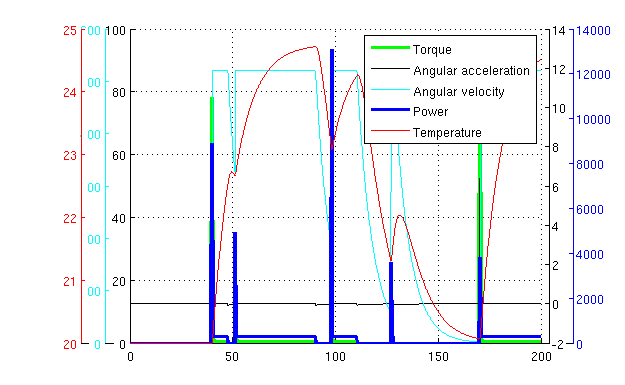
\includegraphics[width=\columnwidth]{simulation-processed}
  		\caption{\lstopar{TODO}}
  		\label{fig:simulation}
	\end{subfigure}
	\begin{subfigure}{.48\columnwidth}
	  	\centering
	  	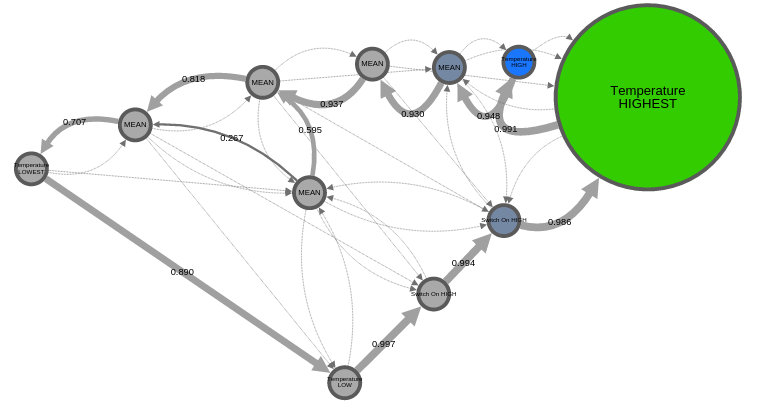
\includegraphics[width=\columnwidth]{model-motor-simulated}
	  	\caption{\lstopar{TODO}}
	  	\label{fig:example-motor}
	\end{subfigure}
\end{figure}

To conduct the experiment we generated two dataset: a training set and a test set. Both datasets
contained $200k$ observations. We built the StreamStory model with 20 lowest-level states on the training set using two attributes:
angular velocity and temperature. The training dataset was then replayed through the model and the
models next state predictions were compared to the actual next state counts. The mean average 
error calculated was $0.05$ or 5\%.

In another experiment we tested the models predictive power. Two StreamStory models were built: (a) one 
model using the same attributes as in the first experiment, while in the second model (b), we used
the logical motor on signal to model state transitions. The models were trained on the same dataset
as in the first experiment. Before the process jumped, we extracted the next state probabilities
and used the state with the highest probability as the predicted next state. We then computed
the prediction accuracy as the ratio between the number of correct prediction and the total number
of jumps (total number of predictions). In this experiment model (a) scored $0.845$ while model
(b) scored $0.904$.


\subsection{Weather Data}
\label{sec:experiments-weather}

The example below shows our model generated on monthly rainfall and temperature data
collected over the course of 20 years between 1920 and 1940 in Nottingham England.

\begin{figure}[h!]
	\centering
	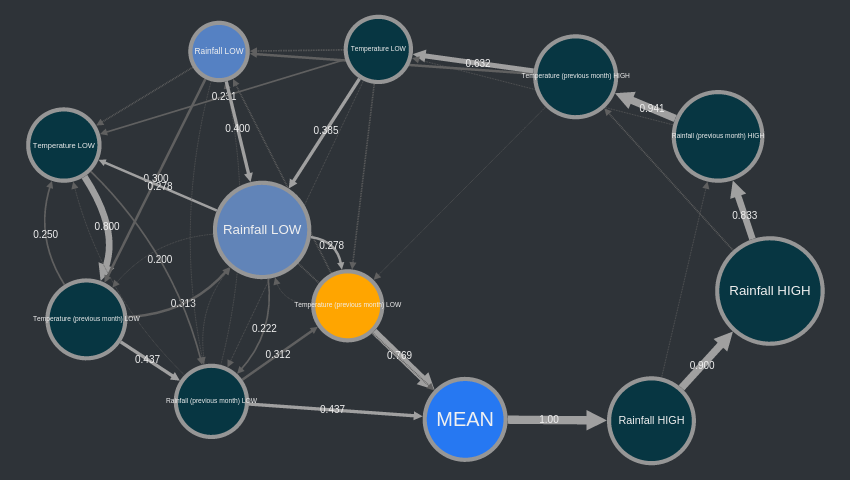
\includegraphics[width=\columnwidth]{example-weather}
	\caption{Qualitative representation of temperature and rainfall data collected over the course of 20 years.}
	\label{fig:example-weather}
\end{figure}

The model was generated using the raw rainfall and temperature data, but each feature vector includes
the rainfall and temperature of the previous month. The states on the right hand side represent the 
summer states, while the states on the left represent winter states. The yearly timeline flows in the
counter clockwise direction with the spring states residing on the bottom of the figure and the autumn
states on the top.

Interestingly, in this dataset, the rainfall and temperature are very highly correlated and the auto naming feature
choose high rainfall as the most significant feature of the summer states. This correlation can be seen
from the attribute histogram shown in Figure \ref{fig:histograms-summer}.

\begin{figure}[h!]
	\centering
	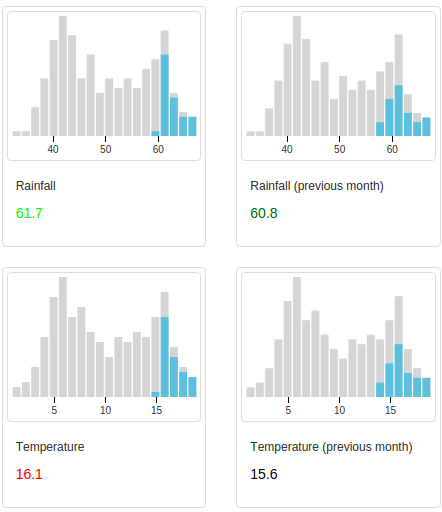
\includegraphics[width=0.5\columnwidth]{histograms-summer}
	\caption{\lstopar{TODO caption}}
	\label{fig:histograms-summer}
\end{figure}

\subsection{GPS Data}

The second example was created using raw GPS coordinates collected using a smartphone between \textcolor{red}{X} and \textcolor{red}{Y}.
The data represents the everyday movement of a European computer science researcher. Figure \ref{fig:example-geo}
shows our qualitative representation of this data on a high level with 8 state.

\begin{figure}[h!]
	\centering
	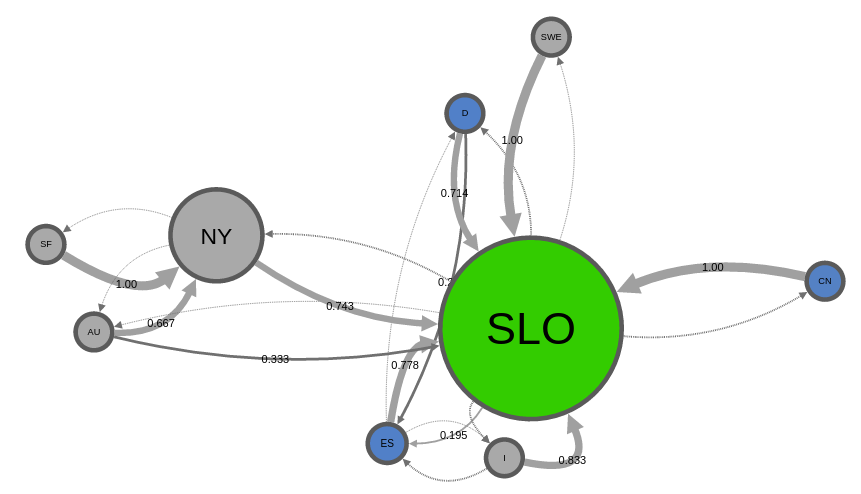
\includegraphics[width=\columnwidth]{geo-states}
	\caption{\lstopar{TODO caption}}
	\label{fig:example-geo}
\end{figure}

From the figure, we can see that the system was able to identify the most typical locations of this persons
movements. Most of the time they spend in central EU including two small states on the bottom and right
representing southern Europe and India where they went for vacation. On the European continent, the system
also identified Germany and Sweden where the person frequently attends meetings or stays for a short while
during a connecting flight. The states on the left represent the USA with the largest state representing New
York city where the person spent the 2014 summer and the smaller states representing San Francisco and Austin,
Texas.

\subsection{Traffic Data}

\begin{figure}[h!]
	\centering
	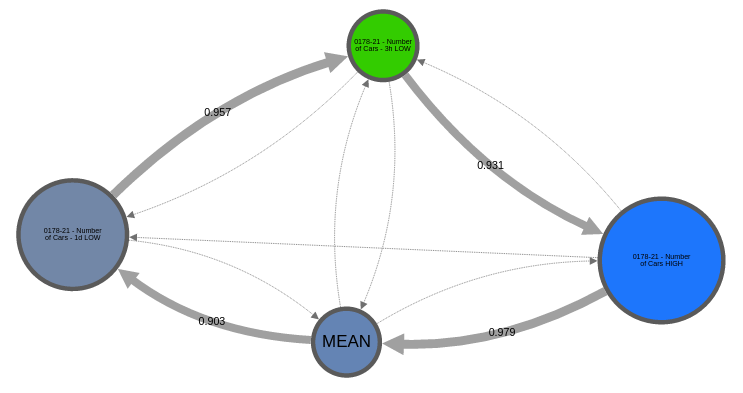
\includegraphics[width=\columnwidth]{example-traffic}
	\caption{\lstopar{TODO caption}}
	\label{fig:example-traffic}
\end{figure}

\subsection{Domain Experts}